\documentclass[tikz,border=10pt]{standalone}
\usepackage{tikz}
\usetikzlibrary{scopes}
\usepackage{verbatim}
\usetikzlibrary{calc,angles,patterns,quotes}
\usepackage{pgfplots}
\usepackage{pgf}
\pgfplotsset{compat=newest}
\pgfplotsset{plot coordinates/math parser=false}


\begin{document}

\def\iangle{35} % Angle of the inclined plane
\def\down{-90}
\def\arcr{0.5cm} % Radius of the arc used to indicate angles
\def\ang{30}
\def\rodlength{1}
\def\soundspeed{1}

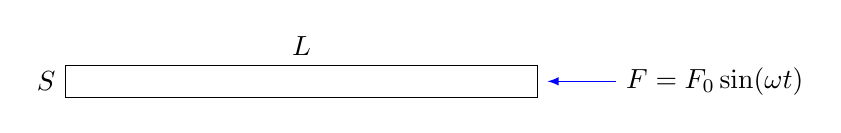
\begin{tikzpicture}[
    force/.style={>=latex,draw=blue,fill=blue},
    axis/.style={densely dashed,gray},
    M/.style={rectangle,draw,fill=lightgray,minimum size=0.5cm,thin},
    m/.style={rectangle,draw=black,fill=lightgray,minimum size=0.3cm,thin},
    plane/.style={draw=black,fill=blue!10},
    string/.style={draw=red, thick},
    pulley/.style={thick}
]


   
    % object and forces acting on it
    \draw (0cm, 0cm) rectangle ++(6cm, 0.4cm) -- ++(0, -0.2cm) node (right_edge){};
    \node[anchor=south] at (3cm, 0.4cm) {$L$};
    \node[anchor=east] at (0cm, 0.2cm) {$S$};

    \draw[force,>=latex,<-] (right_edge) -- ++(1, 0) node[right] {$F=F_0 \sin (\omega t)$};
   


\end{tikzpicture}


%% plot function
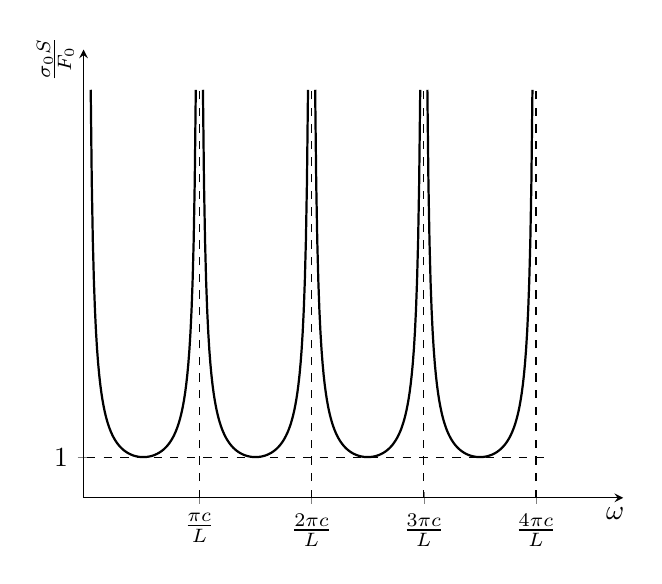
\begin{tikzpicture}[
    force/.style={>=latex,draw=blue,fill=blue},
    axis/.style={densely dashed,gray},
    M/.style={rectangle,draw,fill=lightgray,minimum size=0.5cm,thin},
    m/.style={rectangle,draw=black,fill=lightgray,minimum size=0.3cm,thin},
    plane/.style={draw=black,fill=blue!10},
    string/.style={draw=red, thick},
    pulley/.style={thick}
]


   
\begin{axis}[  
    axis x line=bottom,
    axis y line=left,
    xlabel={$\omega$},
    x label style={at={(axis description cs:0.95, 0)},anchor=north west}, 
    y label style={at={(axis description cs:0, 1.05)},anchor=south east}, 
    ylabel={$\frac{\sigma_0 S}{F_0}$},
    xtick={3.14, 6.28, 9.42, 12.56  },
    xticklabels={$\frac{\pi c}{L}$,$\frac{2\pi c}{L}$,$\frac{3\pi c}{L}$,$\frac{4\pi c}{L}$},
    ytick={1},
    yticklabels={1},
    ymin=0, ymax=11, xmax=15, xmin=-0.1]

    \addplot[domain=0.1:3.04, samples=100, thick] {1 / abs(sin((x / 3.14) * 180))};
    \addplot[dashed] coordinates {(3.14, 0) (3.14, 10)};
    \addplot[domain=3.24:6.18, samples=100, thick] {1 / abs(sin(((x  - 3.14) / 3.14) * 180))};
    \addplot[dashed] coordinates {(6.28, 0) (6.28, 10)};
    \addplot[domain=6.38:9.32, samples=100, thick] {1 / abs(sin(((x  - 3.14 * 2) / 3.14) * 180))};
    \addplot[dashed] coordinates {(9.42, 0) (9.42, 10)};
    \addplot[domain=9.52:12.46, samples=100, thick] {1 / abs(sin(((x  - 3.14 * 3) / 3.14) * 180))};
    \addplot[dashed] coordinates {(12.56, 0) (12.56, 10)};
    \addplot[dashed] coordinates {(0, 1) (13, 1)};
\end{axis}   


\end{tikzpicture}



\end{document}
